\section{Programming using packet transactions}
\label{s:transactions}
\begin{figure*}[!t]
\begin{minipage}{0.6\textwidth}
\begin{small}
\begin{lstlisting}[style=customc]
#define NUM_FLOWLETS    8000
#define THRESHOLD       5
#define NUM_HOPS        10

struct Packet {
  int sport;
  int dport;
  int new_hop;
  int arrival;
  int next_hop;
  int id; // array index
};

int last_time [NUM_FLOWLETS] = {0};
int saved_hop [NUM_FLOWLETS] = {0};

void flowlet(struct Packet pkt) {
  pkt.new_hop = hash3(pkt.sport,
                      pkt.dport,
                      pkt.arrival)
                % NUM_HOPS;

  pkt.id  = hash2(pkt.sport,
                  pkt.dport)
            % NUM_FLOWLETS;

  if (pkt.arrival - last_time[pkt.id] 
      > THRESHOLD) 
  { saved_hop[pkt.id] = pkt.new_hop; }

  last_time[pkt.id] = pkt.arrival;
  pkt.next_hop = saved_hop[pkt.id];
}
\end{lstlisting}
\end{small}
\end{minipage}
%
\vrule\quad
%
\begin{minipage}{0.4\textwidth}
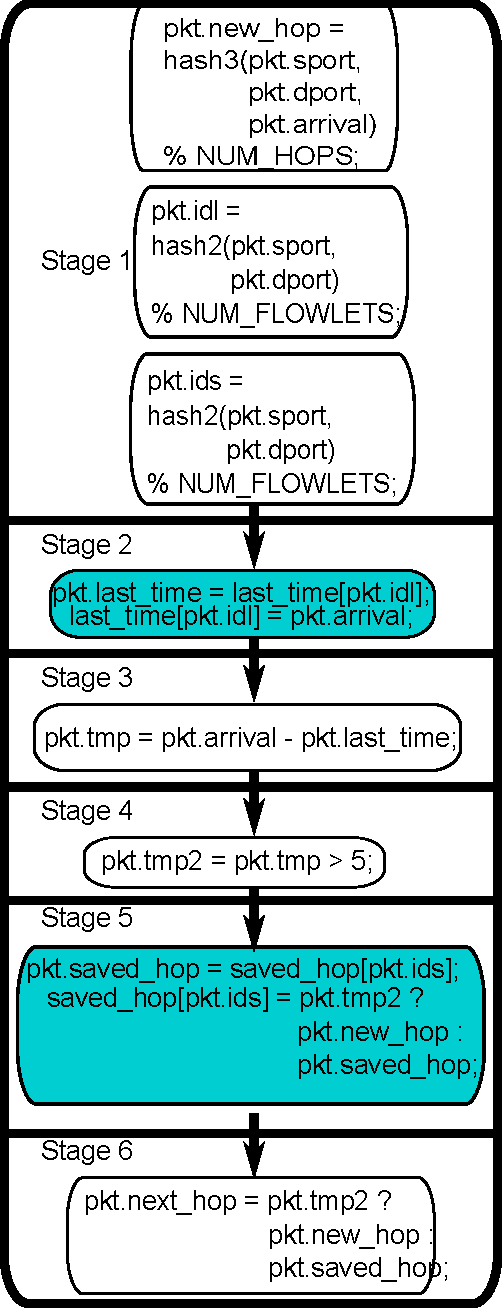
\includegraphics[width=0.8\columnwidth]{pipe.pdf}
\end{minipage}
\caption{\small (a) Flowlet switching written in \pktlanguage (left);
(b) Compiled 6-stage pipeline in \absmachine implementing (a).  Control flows
from top to bottom. Atoms manipulating state are shaded in blue (right).}
\label{fig:flowlet}
\end{figure*}

We now illustrate programming using packet transactions in \pktlanguage, using
flowlet switching~\cite{flowlets} as an example. Flowlet switching is a
load-balancing algorithm that sends bursts of packets (called flowlets) from a
TCP flow on different paths, provided the bursts are separated by a large
enough interval in time to ensure packets do not arrive out of order at the TCP
receiver. Figure~\ref{fig:flowlet} shows how flowlet switching is expressed in
\pktlanguage. For simplicity, the example hashes only the source and
destination ports; it is easy to extend this to the full 5-tuple.

This example demonstrates the core language constructs in \pktlanguage. All
packet processing happens in the context of a packet transaction (the function
\texttt{flowlet} on line 17), a C function taking a C struct as an argument.
The struct declares the fields in a packet (lines 5--12)\footnote{We use fields
to refer to both packet headers such as source port (sport) and destination
port (dport) and packet metadata (id).} that can be referenced by the function
body (lines 18--32).  In addition, the function body can reference state
variables that represent persistent state stored on the switch. These are
declared as global variables (e.g. \texttt{last\_time} and \texttt{saved\_hop}
on lines 14 and 15).

Conceptually, the packet transaction function modifies its packet argument in
place until the end of the function body, before processing the next packet.
\pktlanguage forbids return statements implying that execution will always end
at the end of the function body. The function body may also call
\textit{intrinsics} such as \texttt{hash2} on lines 23 and \texttt{hash3} on
line 18.  Intrinsics are hardware primitives provided by the abstract machine
that aren't interpreted by \pktlanguage. The \pktlanguage compiler uses an
intrinsic's signature to infer dependencies and supplies a canned run-time
implementation, but otherwise doesn't interpret or analyze intrinsics. The
packet transaction's body is written in a constrained subset of C
(Table~\ref{tab:restrict}).

\begin{table}
  \begin{tabular}{|p{0.05\columnwidth}|p{0.8\columnwidth}|}
    \hline
    \# & Restriction \\
    \hline
    1 & No iteration (while, for, do-while).\\
    \hline
    2 & No switch, goto, return, break, or continue.\\
    \hline
    3 & No pointers.\\
    \hline
    4 & No dynamic memory allocation / heap.\\
    \hline
    5 & Array index must be constant over the duration of a packet.\\
    \hline
    6 & No access to packet data.\\
    \hline
  \end{tabular}
  \caption{Restrictions in \pktlanguage}
  \label{tab:restrict}
\end{table}

Arrays can be used as state variables alone (not packet fields), but with
restrictions. While a packet transaction's body is being executed for a
specific packet, all accesses to an array variable must use the same index. For
subsequent packets, this index can be different. For instance, all accesses to
the array \texttt{last\_time} use the index \texttt{pkt.id}, which is constant
for each packet, but changes from one packet to the next. This restriction
simplifies the treatment of arrays in the compiler, while still allowing us to
express several data-plane algorithms of practical interest.

These restrictions seem severe at first glance, but are required to provide
deterministic performance guarantees. Memory allocation, unbounded iteration
counts, and unrestricted control transfer all cause variable run-time
performance. These are also precisely the restrictions in \pktlanguage relative
to languages like Click~\cite{click} that target general-purpose software
routers with greater flexibility and more variable performance.

When compiled to a \absmachine machine (\S\ref{s:absmachine}), the \pktlanguage
compiler converts the code in Figure~\ref{fig:flowlet}a into the pipelined form
shown in Figure~\ref{fig:flowlet}b. Today, programmable switch chips are
programmed by manually specifying low-level configurations resembling
Figure~\ref{fig:flowlet}b using a language like P4. \pktlanguage's compiler
automates this process.
